\documentclass{beamer}

\usepackage{graphicx}
\graphicspath{ {./images/} }

%\usetheme{Madrid}
%\usetheme{Warsaw}
\usetheme{Copenhagen}

%\setbeamertemplate{footline}[frame number]{}
\setbeamertemplate{navigation symbols}{\insertframenumber/\inserttotalframenumber}

\title[Logistical Optimisation for Offshore Windfarms]{Simulation and Optimisation of Offshore Renewable Energy Arrays for Minimal Life-Cycle Costs}

\author{Robin Kuipers}

\date{November 12, 2019}

\begin{document}

\begin{frame}
  \titlepage
\end{frame}

\begin{frame}{The problem}
  \begin{itemize}
  	\item Focus on modern windfarms in the North Sea
  	\item Optimize logistics of operations on offshore windfarms (OWFs) in each phase of the life-cycle:
  	\begin{itemize}
  		\item Installation
  		\item Maintenance
  		\item Decommission
  	\end{itemize}
  	\item Various logistical decisions come into play
  	\item Small optimisations can have significant effects on costs
  	\item Methods used are optimisation and simulation
  \end{itemize}
\end{frame}


\begin{frame}{Key challenges}
  \begin{itemize}
  	\item Long lead-up times
  	\item Strong maritime weather
  	\item Many different types of decisions
  	\item Differences between locations
  	\item Phases are not independent
  \end{itemize}
\end{frame}


\begin{frame}{Existing literature}
   \begin{itemize}
  	\item Various attempts to improve the installation phase, through integer programming and local search, combined with simulation
  	\item A lot of research has been done in various areas of maintenance, including supply chain management, mitigating failure rate, condition based maintenance
  	\item Not a lot of research has been done on decommission projects, but they are similar in structure to installation projects
  	\item No research at all has been found that looks at the entire life-cycle and how the different phases affect each other
  \end{itemize}
\end{frame}


\begin{frame}{Research objectives}
  \begin{itemize}
  	\item Design an integrated optimisation and simulation model spanning the entire life-cycle of an Offshore Wind Farm, based on sub-models for each phase of the life-cycle.
  	\item Sub-objectives:
  	\begin{itemize}
  		\item Design an integrated optimisation and simulation model for the installation projects of an OWF. 
  		\item Design an integrated optimisation and simulation model for the maintenance projects of an OWF. 
  		\item Design an integrated optimisation and simulation model for the decommissioning projects of an OWF. 
  	\end{itemize}
  \end{itemize}
\end{frame}


\begin{frame}{Current Progress}
   \begin{itemize}
  	\item Reviewed a large part of the literature, primarily on installation projects and secondarily on maintenance projects and general non-deterministic scheduling and robust optimisation
	\item Specified research area and objectives
  	\item Laid the foundations for a decision support tool suited to analyse and optimise schedules for any phase of the life-cycle, based on project-specific characteristics
  	\item Planned the interactions between my various models	
  \end{itemize}
\end{frame}


\begin{frame}{Model interactions - 1}
\begin{columns}
	\begin{column}{0.5\textwidth}
		\begin{enumerate}
			\item Optimisation Model (OM) gets info about the site and task structure
			\item OM calculates new/improves existing schedule and sends it to the Simulation Model (SM)
			\item SM runs simulations with the schedule, returns metrics back to OM
			\item OM determines that end conditions are met or returns to step 2
		\end{enumerate}
	\end{column}

	\begin{column}{0.5\textwidth}
		\begin{figure}[t]
 			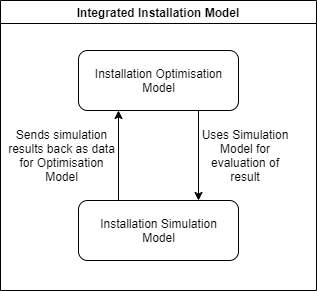
\includegraphics[width=\textwidth]{Installation}
			\centering
		\end{figure}
	\end{column}
\end{columns}
\end{frame}


\begin{frame}{Model interactions - 2}
\begin{figure}[t]
  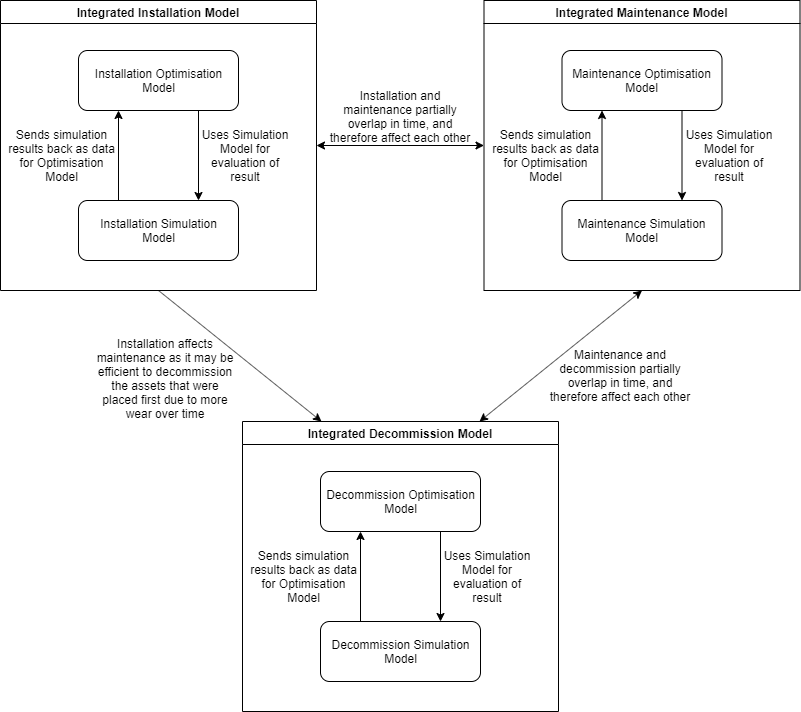
\includegraphics[width=0.8\textwidth]{flowchart}
\centering
\end{figure}
\end{frame}


\begin{frame}{Future Work}
   \begin{itemize}
  	\item Develop full models for each phase of the life-cycle
  	\item Determine specific interactions between the phases
  	\item Implement models in the tool, develop it further for full commercial functionality
  	\item Validate and test the tool (and underlying models) using real(istic) data
  \end{itemize}
  \pause
  \bigskip
  \begin{center}
  Thank you for listening, any questions?
  \end{center}
\end{frame}

\end{document}


